\chapter{Evaluation}\label{chap:evaluation}
\ifpdf
    \graphicspath{{Evaluation/Figs/Raster/}{Evaluation/Figs/PDF/}{Evaluation/Figs/}}
\else
    \graphicspath{{Evaluation/Figs/Vector/}{Evaluation/Figs/}}
\fi

To evaluate the performance of FAT-Pointer based range addresses a sample implementation we used
the morello board with CheriBSD's Benchmark ABI\cite{noauthor_benchmark_nodate} compilation mode for accurate performance recordings. 
The evaluation is to identify CheriBSD's default memory allocator SnMalloc\cite{lietar_snmalloc_2019} against the prototype memory 
allocator using the contribution of this paper in terms of: 
To assess the performance of FAT-Pointer-based range addressing in the sample implementation, we utilized the 
Morello board running CheriBSD in Benchmark ABI compilation mode to ensure precise performance measurements. 
The evaluation focuses on comparing CheriBSD's default memory allocator, SnMalloc, against the prototype 
memory allocator developed in this study, with particular attention to the following aspects:

\begin{table}[!ht]
  \centering
  \begin{tabular}{|l|l|l|l|l|}
  \hline
      Metric name & type of graph & tool used & x axis & y axis \\ \hline
      DTLB L1 read & line graph & Pmcstat & Time & DTLB L1 reads (each second) \\ \hline
      DTLB L2 read & line graph & Pmcstat & Time & DTLB L2 reads (each second) \\ \hline
      DTLB walk & line graph & Pmcstat & Time & DTLB Walks (each second) \\ \hline
      L1 cache miss & line graph & Pmcstat & Time & L1 cache miss (each second) \\ \hline
      Wall clock run time & bar graph & time & Benchmarks & Time \\ \hline
  \end{tabular}
  \caption{Metrics evaluated}
\end{table}

\section{Benchmarks used}
To conduct the evaluations, we utilized the COZ\cite{curtsinger_coz_2015} benchmark suite, a well-regarded tool specifically designed 
to measure and analyze performance improvements in concurrent programs. The COZ benchmark suite provides a
robust framework for identifying bottlenecks and evaluating the performance impact of various optimization
techniques. By leveraging COZ, developers can gain precise insights into the efficiency and scalability of
their concurrent code, making it an ideal choice for rigorous performance analysis.

From the extensive set of benchmarks provided by COZ, we selected three representative C programs. 
These programs were chosen based on their relevance to common concurrent programming patterns and
their ability to effectively demonstrate the strengths and weaknesses of different optimization 
strategies. The selected programs cover a range of concurrency scenarios, ensuring a comprehensive
evaluation of performance improvements.

By implementing these modifications, we ensured that the selected C programs not only adhered to
CHERI's security model but also maintained their functional and performance characteristics. 
This allowed us to effectively use the COZ benchmark suite to analyze the performance in a CHERI-enhanced environment.

\begin{figure}[h]
  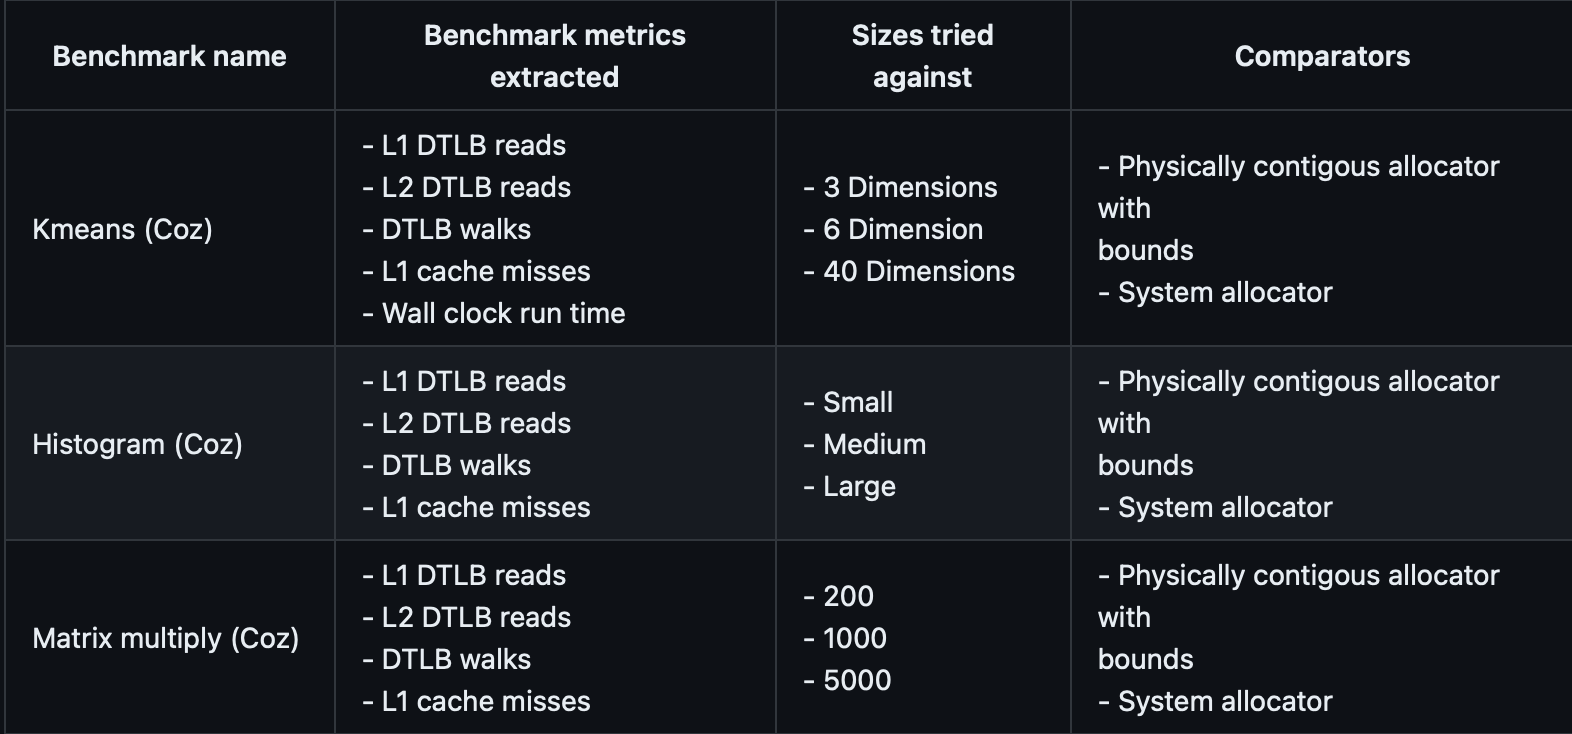
\includegraphics[width=0.8\textwidth]{diagrams/expirement-runs.png}
  \caption{C programs evaluated}
\end{figure}

\subsection{DTLB L1 reads}
% L1 TLB graphs
\begin{figure}
  \begin{subfigure}{\linewidth}
  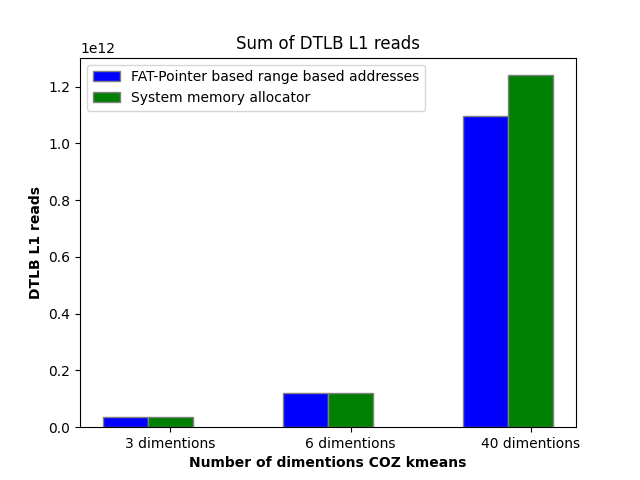
\includegraphics[width=.5\linewidth]{l1-tlb-kmeans.png}\hfill
  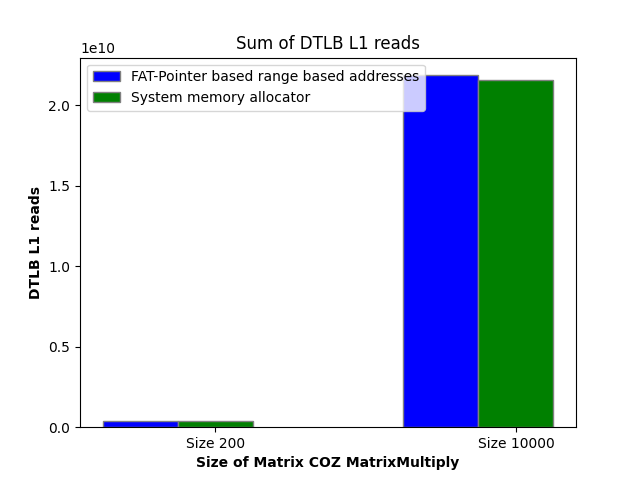
\includegraphics[width=.5\linewidth]{l1-tlb-matrixmultiply.png}\hfill
  \includegraphics[width=.5\linewidth]{l1-tlb-histogram.png}
\end{subfigure}
\caption{DTLB L1 reads}
\label{fig:TLBl1}
\end{figure}
The Graphs above represent the DTLB L1 reads which is a Performance counter from the ARM specs. 
The counter increments for every Memory-read or Memory-write operation that necessitates an 
access to the Level 1 data or unified Translation Lookaside Buffer (TLB). 
Each access to a TLB entry is counted including multiple accesses caused by single instructions.

\subsection{DTLB L2 reads}
% L2 TLB graphs
\begin{figure}
  \begin{subfigure}{\linewidth}
    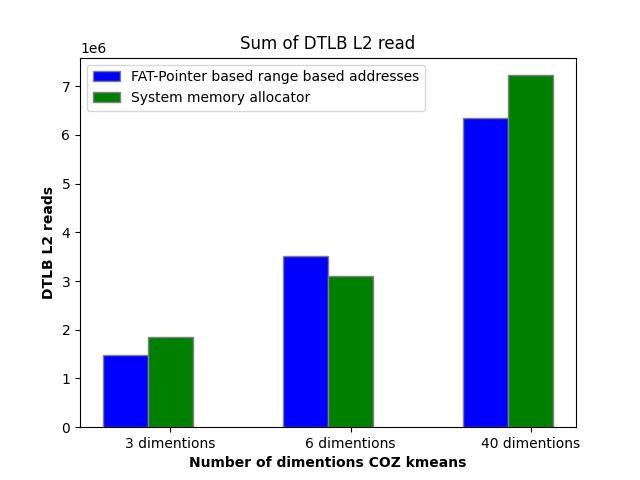
\includegraphics[width=.5\linewidth]{l2-tlb-kmeans.png}\hfill
    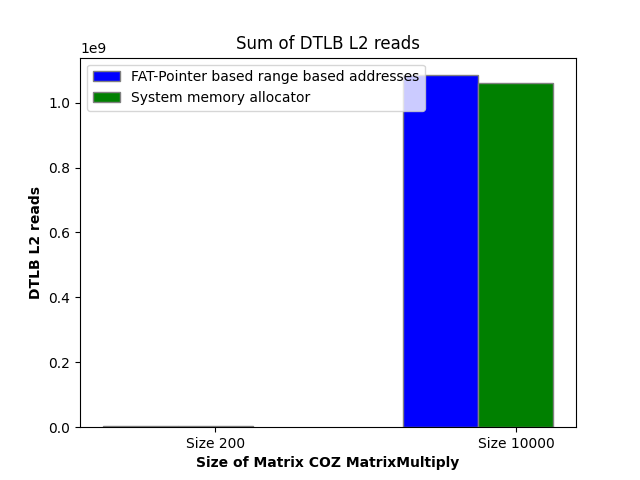
\includegraphics[width=.5\linewidth]{l2-tlb-matrixmultiply.png}\hfill
    \includegraphics[width=.5\linewidth]{l2-tlb-histogram.png}
\end{subfigure}
\caption{DTLB L2 reads}
\label{fig:TLBl2}
\end{figure}
Similar to how L1 TLB reads are counted, DTLB L2 counts every read operation that accesses the 
Level 2 data or unified TLB. Each time there is a read to an entry in the Level 2 TLB, 
it is counted by the ARM performance counter. 

% DTLB walks
% - Explain how the stat is calculated 
% - Fix older paragraphs 

\subsection{DTLB walks}
\begin{figure}
  \begin{subfigure}{\linewidth}
    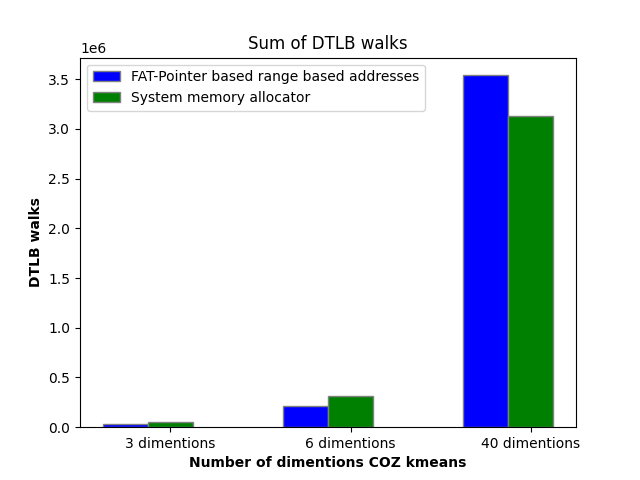
\includegraphics[width=.5\linewidth]{tlb-walk-kmeans.png}\hfill
    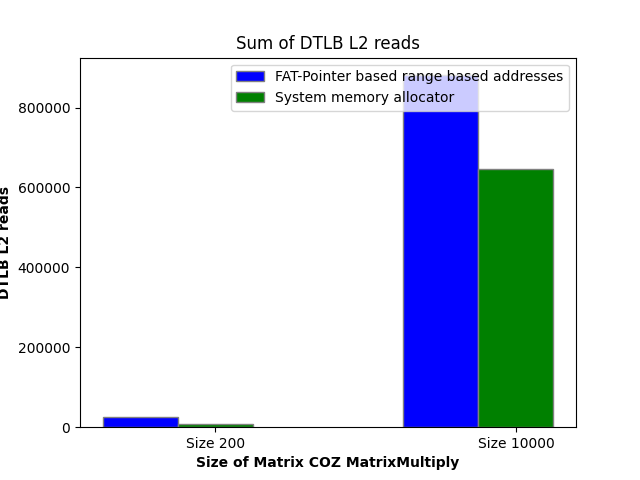
\includegraphics[width=.5\linewidth]{tlb-walk-matrixmultiply.png}\hfill
    \includegraphics[width=.5\linewidth]{tlb-walk-histogram.png}
\end{subfigure}
\caption{DTLB Walks}
\label{fig:TLBWalk}
\end{figure}

The DTLB walk counter counts each Memory-read operation or Memory-write operation that causes a 
TLB access to at least the Level 2 data or unified TLB.
Each access to a TLB entry is counted including refills 
of Level 1 TLBs.

% L1 cache miss
\subsection{L1 cache miss}
\begin{figure}
  \begin{subfigure}{\linewidth}
    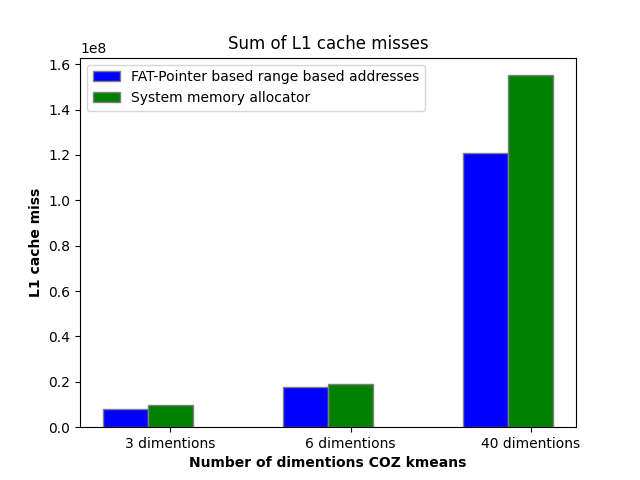
\includegraphics[width=.5\linewidth]{l1-miss-kmeans.png}\hfill
    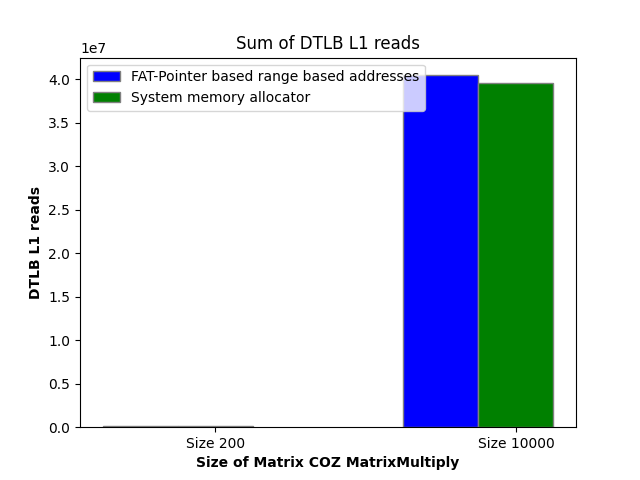
\includegraphics[width=.5\linewidth]{l1-miss-matrixmultiply.png}\hfill
    \includegraphics[width=.5\linewidth]{l1-miss-histogram.png}
\end{subfigure}
\caption{L1 Cache misses}
\label{fig:L1CacheMiss}
\end{figure}
L1 cache miss counter counts each Memory-read operation to the Level 1 data or unified cache counted by L1 cache miss counter that incurs additional latency because it returns data from outside of the Level 1 data or unified cache of this PE.
The event indicates to software that the access missed in the Level 1 data or unified cache and might have a significant performance impact due to the additional latency compared to the latency of an access that hits in the Level 1 data or unified cache.
\newline
% • Accesses where the additional latency is unlikely to be significantly performance-impacting. For example, if the access hits in another cache in the same local cluster, and the additional latency is small when compared to a miss in all Level 1 caches that the access looks up in and results in an access being made to a Level 2 cache or elsewhere beyond the Level 1 data or unified cache.
% • A miss that does not cause a new cache refill but is satisfied from a previous miss.

% The Benchmark results indicates bugs in the sample FAT-Pointer based range address prototype
% memory allocator. This is an ongoing evaluation and results provided above are a snapshot of the
% latest results. For the use case of the L2 TLB reads for the FAT-Pointer based range address prototype
% show that there are reads. This means that there are bugs in the implementation since all reads should 
% be through the L1TLB since for the program memory is pre-allocated as single physically contgious page. 

\section{Analysis}

The benchmark results indicate the presence of bugs in the sample FAT-Pointer based range address prototype memory allocator. This evaluation is ongoing, and the 
results provided in figures \ref{fig:TLBl1}, \ref{fig:TLBl2}, \ref{fig:TLBWalk} and \ref{fig:L1CacheMiss} represent a snapshot of the latest findings. Specifically, for the use case of Level 2 Translation Lookaside Buffer (L2 TLB) reads, 
the FAT-Pointer based range address prototype shows occurrences of reads from the L2 TLB. This indicates the presence of implementation bugs, 
as all reads should be managed through the Level 1 Translation Lookaside Buffer (L1 TLB), given that the program memory is pre-allocated as a single 
physically contiguous page.
\newline

In a correctly functioning system, the L1 TLB should handle all memory accesses, ensuring efficient translation and minimizing latency. 
The detection of L2 TLB reads suggests that there are flaws in the current implementation, potentially in the memory allocation or 
address translation mechanisms. These bugs need to be addressed to achieve the intended performance and correctness of the 
FAT-Pointer based range address prototype memory allocator. Further investigation and debugging are required to 
identify the exact causes and rectify these issues to ensure that all memory accesses are correctly routed 
through the L1 TLB as designed.
\newline

The ContigMalloc function in CheriBSD is designed to allocate contiguous blocks of physical memory. In theory, this should result in a single large block of memory 
that is efficiently handled by the L1 cache, reducing cache misses and improving performance. However, the observed behavior suggests otherwise.
\newline

A slab allocator divides memory into small, fixed-size chunks or "slabs" for allocation. While this can be efficient for managing 
objects of uniform size, it can lead to increased cache misses if objects are not optimally aligned or if there is fragmentation. 
The slab allocation pattern can cause data to be scattered across different cache lines, leading to inefficient cache usage.
\newline

In the k-means C program, which involves intensive computation and frequent memory accesses, L1 cache efficiency is 
crucial for performance. The presence of significant L1 cache misses indicates that the memory allocation is not as 
contiguous as expected. Instead, it suggests that the memory may be fragmented or scattered, similar to what happens with a slab allocator.
\newline

Given the behavior of ContigMalloc and the observed cache performance, it is speculated that ContigMalloc may be 
functioning in a manner similar to a slab allocator under the hood. This could involve internal mechanisms that 
break down the large contiguous allocation request into smaller chunks or slabs for management, inadvertently 
causing the observed L1 cache misses.
\newline

The deviation from truly contiguous allocation impacts the performance of programs like k-means, which rely on efficient 
memory access patterns. L1 cache misses can significantly slow down computation, as accessing data from higher-level 
caches or main memory introduces additional latency. To confirm this hypothesis, further investigation is needed. 
This includes analyzing the internal implementation of ContigMalloc to understand its allocation strategy, 
profiling the memory allocation patterns and cache usage in detail, and conducting controlled experiments 
to compare the behavior of ContigMalloc with known slab allocators.
\newline

If the hypothesis is confirmed, potential solutions could involve modifying ContigMalloc to ensure truly contiguous 
physical memory allocation, implementing custom memory allocators tailored to the specific needs of high-performance 
applications like k-means, and optimizing the existing allocation strategy to minimize fragmentation and improve cache 
utilization. In summary, while ContigMalloc is intended to provide contiguous memory allocation, its current behavior 
suggests a resemblance to slab allocation, leading to suboptimal L1 cache performance in the k-means C program. 
This calls for a deeper dive into the allocator's implementation and strategic adjustments to achieve the 
desired memory access efficiency.
